
\section{Inference and Hypothesis Test}
一般のモデルにおけるパラメータの推定量として以下の2種類を与える。1つ目は純粋戦略ナッシュ均衡の仮定(以下pure strategy Nash equilibriumを略してPNと呼称する)の下で一致性を持つ推定量である。すなわち$\largestar_m$においては必ず$(0,1), (1,0)$のどちらかが実現するという仮定の下での推定量であり、ここでは\cite{Bresnahan1991}において考案された複数均衡に対して頑健な参入企業数を結果変数として用いた最尤推定を紹介する。この推定量を以下PN推定量と呼ぶ。2つ目に$\largestar_m$において純粋戦略ナッシュ均衡と混合戦略ナッシュ均衡がどのような割合で実現していてもパラメータを一致推定できる頑健な推定量を与える。これを以下ではRobust推定量と呼ぶ。

それぞれの推定量についてデータの種類に応じて2つの推定方法を与える。まず想定するデータセットは、$M$市場に関して$T$期分の2社についての参入結果がデータとして得られている理想的な状況を想定したものである。しかし、\cite{Ciliberto2009a}で扱われるような企業参入に関するデータは$M$市場について1回の参入結果がデータとして得られている場合が多い。また、仮に$M$市場についてそれぞれ複数回の参入結果が得られたとしても、研究者には観測不可能な効用が各回で独立に発生するケースは想定しにくい。同じ市場について複数回の参入結果が得られているのであればその結果は系列相関を持つはずであり、ここで想定するように同じ市場について参入企業数の十分な分散を保証してくれる可能性は低い。そこで2つ目のデータセットとして$M$市場について1回だけ参入結果が得られている状況を想定する。

\subsection{PN推定量}
純粋戦略を仮定した時、$\largestar_m$においては複数の均衡が存在するので単純にプレイヤーの参入結果を結果変数に用いると、すべての事象の実現確率を足すと$1$を超えてしまうため適切な尤度を構成できない。しかし、$\largestar_m$において2つある純粋戦略ナッシュ均衡の結果がどちらも1社のみ参入するという結果であることを利用して、参入した企業の数を結果変数としたBivariate Probitを行うことでパラメータが推定できる。

\subsubsection{$M$市場$T$期データ}
市場$m$に着目する。$t_2^m$を2社がどちらも参入した回数、$t_0^m$をどちらも参入しなかった回数とする。企業$i$について参入することが支配戦略となる確率と参入しないことが支配戦略となる確率とを$(q_i^1, q_i^0)$で表記する。$\phi(\cdot),\ \Phi(\cdot)$をそれぞれ標準正規分布の確率密度関数、確率分布関数とした時これは以下のように書ける。
\begin{align*}
\begin{cases}
	q_i^1 = \int_{-{\bf x}_{m, i}^{'} \beta_i - \delta_i}^{\infty} \phi(\epsilon_i) \mathrm{d}\epsilon_i = \Phi({\bf x}_{m, i}^{'} \beta_i + \delta_i)\\[10pt]
	q_i^0 = \int_{-\infty}^{-{\bf x}_{m, i}^{'} \beta_i} \phi(\epsilon_i) \mathrm{d}\epsilon_i = \Phi(-{\bf x}_{m, i}^{'} \beta_i)
\end{cases}
\end{align*}

従って市場$m$におけるデータを$D^m$、パラメータの組を$\theta$で表記すると対数尤度は以下のようである。またこれによって得た推定量を$\theta^P$で表記する。
\begin{align*}
	&\sum_{m = 1}^M g(D^m \mid \theta)\\[10pt]
	&\text{where}\quad g(D^m \mid \theta) = t_2^m\ {\rm log} (q_1^1 q_2^1) + t_0^m\ {\rm log} (q_1^0 q_2^0) + (T - t_2^m - t_0^m)\ {\rm log} (1- q_1^1 q_2^1 - q_1^0 q_2^0)
\end{align*}

\subsubsection{$M$市場データ}
市場$m$に着目する。実現した参入企業数を$n_m\ \in \left\{ 0,1,2 \right\}$で表記すると、尤度は以下のように書ける。

\begin{align*}
	&\sum_{m = 1}^M h(D^m \mid \theta)\\[10pt]
	&\text{where}\quad h(D^m \mid \theta) = {\bf 1}\left[ n_m = 2 \right]\ {\rm log} (q_1^1 q_2^1) + {\bf 1}\left[ n_m = 0 \right]\ {\rm log} (q_1^0 q_2^0) + {\bf 1}\left[ n_m = 1 \right]\ {\rm log} (1- q_1^1 q_2^1 - q_1^0 q_2^0)
\end{align*}

これよりパラメータの最尤推定量を得る。この推定量を以下$\theta_r^P$と表記する。


\subsection{Robust推定量}
Robust推定量の構成には、一定の条件の下で各市場において企業が$2$社ともに参入する確率と企業が$1$社も参入しない確率との差が$\largestar_m$における均衡選択の仮定によらず一定であることを利用する。

\subsubsection{M市場T期データ}
$\largestar_m$における均衡選択メカニズムとして、$w \in [0,1]$の確率で混合戦略ナッシュ均衡が実現するとする。例えば先のPNの仮定は$w = 0$の場合であると言える。またこのメカニズムに以下の仮定を置く。

\begin{description}
\item[仮定1:uniform equilibrium selection mechanism] $w$は$(\epsilon_1, \epsilon_2)$に依存しない。
\end{description}

ここで$1$社も参入しない確率と両者ともに参入する確率との差分を$\alpha(w)$と書くと、
\begin{align*}
	\alpha(w) = w\ \left\{ G_1 G_2 \left( 1 + \frac{{\bf x}_{m, 1}^{'} \beta_1}{\delta_1} + \frac{{\bf x}_{m, 2}^{'} \beta_2}{\delta_2} \right) + \frac{G_1g_2}{\delta_2} + \frac{G_2g_1}{\delta_1} \right\}
\end{align*}
ただし、
\begin{align*}
\begin{cases}
	G_i =  \Phi({\bf x}_{m, i}^{'} \beta_i) - \Phi({\bf x}_{m, i}^{'} \beta_i  + \delta_i)\\
	g_i = \phi({\bf x}_{m, i}^{'} \beta_i) - \phi({\bf x}_{m, i}^{'} \beta_i  + \delta_i)
\end{cases}
\end{align*}
である。証明はAppendix7.1に載せる。

この時以下の2つが成立する。
\begin{description}
	\item[主張$1$] $\left| \alpha(w) \right|$は$w$についての増加関数である。
	\item[主張$2$] $\forall i \in \left\{ 1,2\right\}$で${\bf x}_{m, i}^{'} \beta_i + \delta_i$が十分に大きいならば$\alpha(1)$を十分0に近づけることができる。
\end{description}

主張1は明らかである。主張2については図1より確認できる。

\begin{figure}[t]
\centering
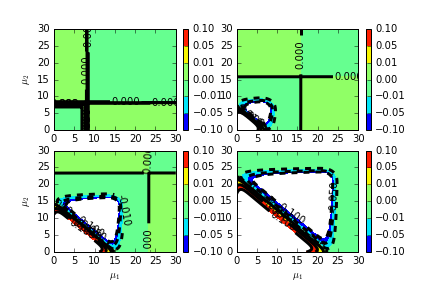
\includegraphics{diff3.png}
\caption{頑健性 左上から順に$\delta = -0.01$, $\delta = -7.4$, $\delta = -15$, $\delta = -22.5$の時の等高線}
\end{figure}

図$1$は$\mu_i = {\bf x}_{m, i}^{'} \beta_i$として、$\delta = \delta_1 = \delta_2$という対称性の仮定の下で各$(\mu_1, \mu_2, \delta)$に対して$\alpha(1)$の値を出力し、$\delta$の値ごとに等高線で表示したものである。図$1$からわかるように$\mu_i + \delta$が両プレイヤーにとって十分大きい領域では$\alpha(1)$が十分小さくなっている。すなわちパラメータとサンプルにこの性質を満たすという仮定を置くと、$\alpha(1)$は図$2$の\textcircled{\scriptsize 2}と\textcircled{\scriptsize 1}の領域の差分と等しいことを意味する。また$\delta_i$についての対称性の仮定を緩めてもこれは同じように成立する。

\begin{figure}[t]
\centering
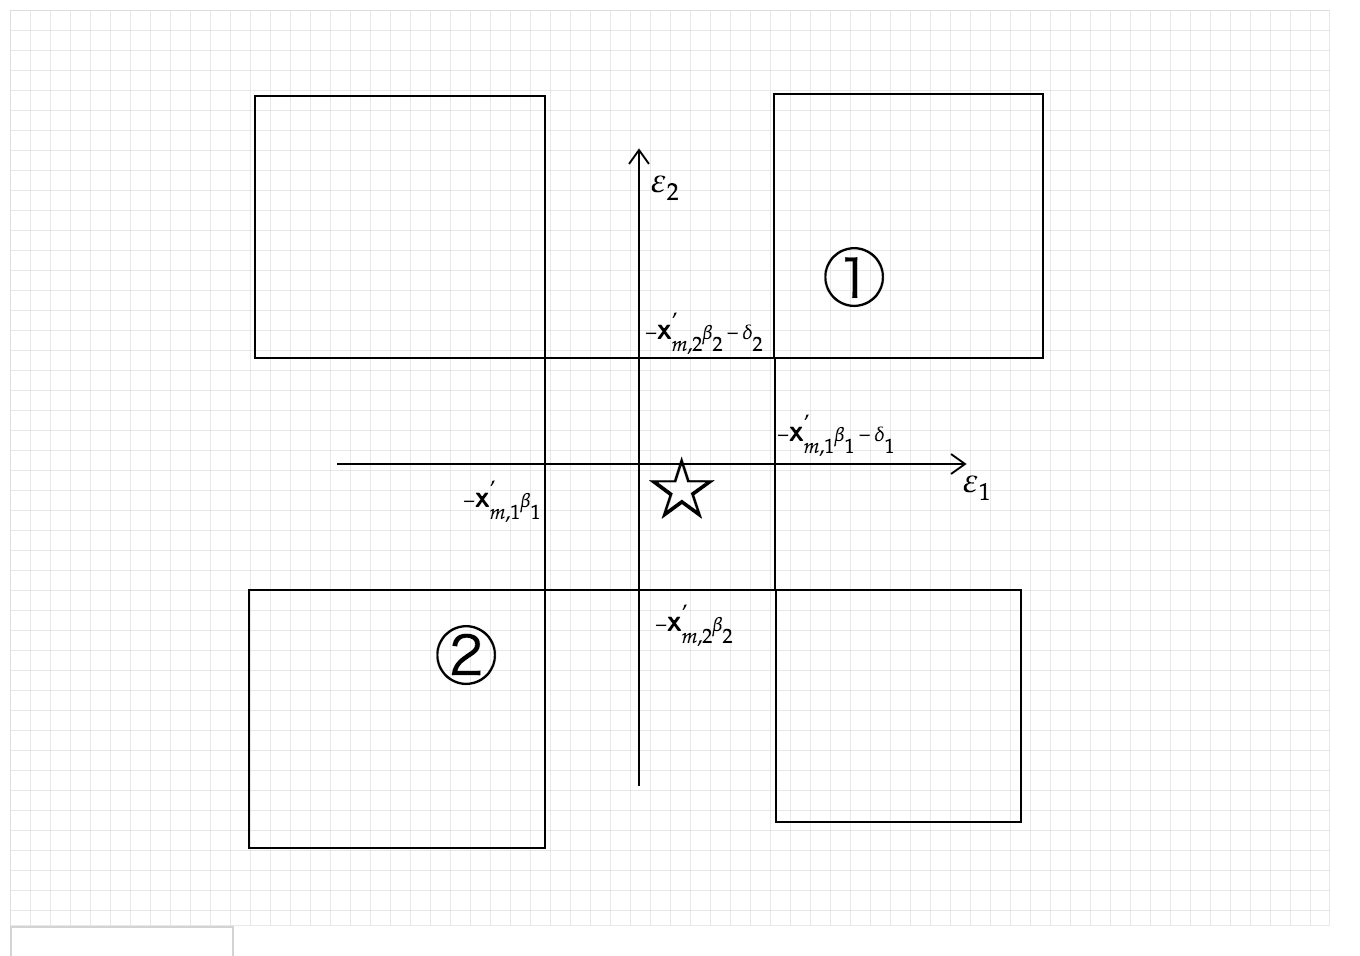
\includegraphics[scale = 0.3]{brgraph.png}
\caption{均衡の分布}
\end{figure}

さらに主張$1$より$\alpha(1)$が十分$0$に近い領域のパラメータセットにおいては他のいかなる$w \in [0,1]$においても十分$0$に近いことがわかる。従って「$\forall i \in \left\{ 1,2\right\}$で${\bf x}_{m, i}^{'} \beta_i + \delta_i$が十分に大きい」という仮定の下では、$\largestar_m$においていかなる均衡選択メカニズムが存在しようと、「$1$社も参入しない確率と両者ともに参入する確率との差分は図$2$の\textcircled{\scriptsize 2}と\textcircled{\scriptsize 1}の領域の差分と等しい」というモーメント条件を用いてパラメータの推定を行うことができる。

以上の議論よりRobust推定量$(\theta^R)$は以下のように定義される。ただし、$p_2^m$は市場$m$において$2$社が共に参入する確率であり、$\hat{p_2^m}$は$T$期のデータからその確率を推定したものである。すなわち$n_m^t$を市場$m$の$t$期目で参入した企業数として$\hat{p_2^m} = \frac{1}{T} \sum_{t = 1}^T {\bf 1}\left[ n_m^t = 2 \right]$である。$p_0^m$と$\hat{p_0^m}$についても同様に定義される。
\begin{align*}
	&\theta^R = \argmin_{\theta} \sum_{m = 1}^M r(\hat{p^m} ; \theta)^2\\[10pt]
	&\text{where}\ r(\hat{p^m} ; \theta) = (\hat{p_2^m} - \hat{p_1^m}) - (q_1^1 q_2^1 - q_1^0 q_2^0)
\end{align*}

識別に関しては以下が成立する。
\begin{description}
	\item[主張3] \cite{Tamer2003a}の除外制約の下でRobust推定量$(\theta^R)$は識別可能である。
\end{description}
証明はAppendix7.2に記す。

\subsubsection{$M$市場データ}
市場$m$に関して$1$回分のデータしか得られていない状況を考える。Robust推定量の構成に必要なのは各市場ごとの$p_2^m,p_0^m$である。$p_2^m,p_0^m$は説明変数の値に依存する関数であることから、多項ロジットで当該関数を推定し、それによって得られる$p_2^m,p_0^m$の予測値を利用することで先と同様の非線形最小二乗推定量を得ることができる。以下これを$\theta_r^R$と表記する。

多項ロジットによって得た$p_2^m,p_0^m$の推定値を$\tilde{p_2^m}, \tilde{p_1^m}$と表記する。図$3$はサンプルデータを用いて実際に推定した$\tilde{p_0^m} - \tilde{p_2^m}$を縦軸に、横軸には同じデータセットから推定した$\hat{p_2^m} - \hat{p_1^m}$をとった散布図である。多項ロジットによって差分がよく推定されていることがわかる。

\begin{figure}[t]
\centering
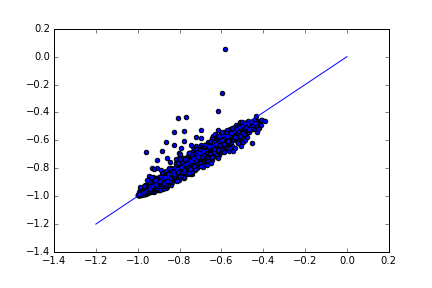
\includegraphics{logit.png}
\caption{多項ロジットによる差分の予測 直線は$\tilde{p_0^m} - \tilde{p_2^m} = \hat{p_2^m} - \hat{p_1^m}$}
\end{figure}

\subsection{Hypothesis Test}
前章で述べた頑健な推定量を用いてハウスマン検定により純粋戦略ナッシュ均衡の仮定に対する仮説検定を行うことを考える。ただし、通常のハウスマン検定では有効推定量を用いるのに対し、\cite{Tamer2003a}で述べられたようにPN推定量は有効推定量ではない。従って非有効推定量同士を用いたハウスマン検定を考える必要があることに注意する。

まず$M$市場$T$期のデータがある状況に対するハウスマン検定統計量を与える。パラメータの真の値を$\theta^0$で表記すると先の2つの推定量について漸近分布は以下で与えられる。

\begin{align*}
	\begin{pmatrix}
	\sqrt{M}(\theta^P - \theta^0)\\[8pt]
	\sqrt{M}(\theta^R - \theta^0)
	\end{pmatrix}\ \xrightarrow{d}\ 
	N\left( \begin{pmatrix}0\\[8pt]0
	\end{pmatrix},\ 
	\begin{pmatrix}
	A_{11} & A_{12}\\[8pt]
	A_{21} & A_{22}
	\end{pmatrix}
	\right)
\end{align*}

ここで$r(\theta) = \frac{1}{M} \sum_m r(\hat{p^m} ; \theta)$として$R(\theta) = \frac{\mathrm{d}r}{\mathrm{d} \theta^{'}}$と置く。このとき、以下の$2$つの行列を用いることで漸近分散を$A S A^{'}$と表すことができる。

\begin{align*}
	S = Var\begin{pmatrix}
	\frac{1}{\sqrt{M}} \sum_m \nabla_{\theta} g(D^m \mid \theta^0)\\[8pt]
	\frac{1}{\sqrt{M}} \sum_m\ r(p^m \mid \theta^0)
	\end{pmatrix},\ 
	A = \begin{pmatrix}
	-E\left[ \nabla_{\theta \theta^{'}}g(D^m \mid \theta^0) \right]^{-1} & 0\\[8pt]
	0 & -\left( R(\theta^0)^{'} R(\theta^0) \right)^{-1} R(\theta^0)^{'}
	\end{pmatrix}
\end{align*}

ここでハウスマン検定統計量$H$は$q = \sqrt{M} (\theta^P - \theta^R)$と置くと以下で定義される。
\begin{align*}
H = q^{'} \left( \hat{Avar\left( q \right)} \right)^{-1} q
\end{align*}
ただし$\hat{Avar\left( q \right)}$は$q$の分散共分散行列の推定値であり、デルタメソッドより以下のように求められる。
\begin{align*}
	\hat{Avar\left( q \right)} = \hat{A_{11}} - \hat{A_{12}} - \hat{A_{21}} + \hat{A_{22}} 
\end{align*}
ここで$\left(\hat{A_{11}},\ \hat{A_{12}},\ \hat{A_{21}},\ \hat{A_{22}} \right)$は各要素のサンプルからの推定値である。帰無仮説は「$\largestar_m$で純粋戦略ナッシュ均衡が常に実現する」であり、帰無仮説の下で$H$は自由度$2K + 2$の$\chi^2$分布に従う。これを利用し有意水準$5\%$の仮説検定を行うことができる。

次に$M$市場について$1$回分の参入結果しかない場合のハウスマン検定統計量を与える。上で述べた理想的なデータセットにおける尤度関数$g$を$h$に変え、さらにRobust推定量における$\hat{p_2^m} - \hat{p_1^m}$を$\tilde{p_0^m} - \tilde{p_2^m}$に置き換える。また各パラメータの推定値に$M$市場データから得られた$\theta_r^P,\ \theta_r^R$を用いることで得られるため詳細は省略する。